\section{Design}
\subsection{Introduction}
This chapter covers project architecture and process flow as well as the math foundations of algorithms used in this project.
The second topic is partly covered in the Background reading chapter, but here there is all the information necessary for understanding.
\subsection{Project architecture and process flow}
\begin{figure}[ht]
    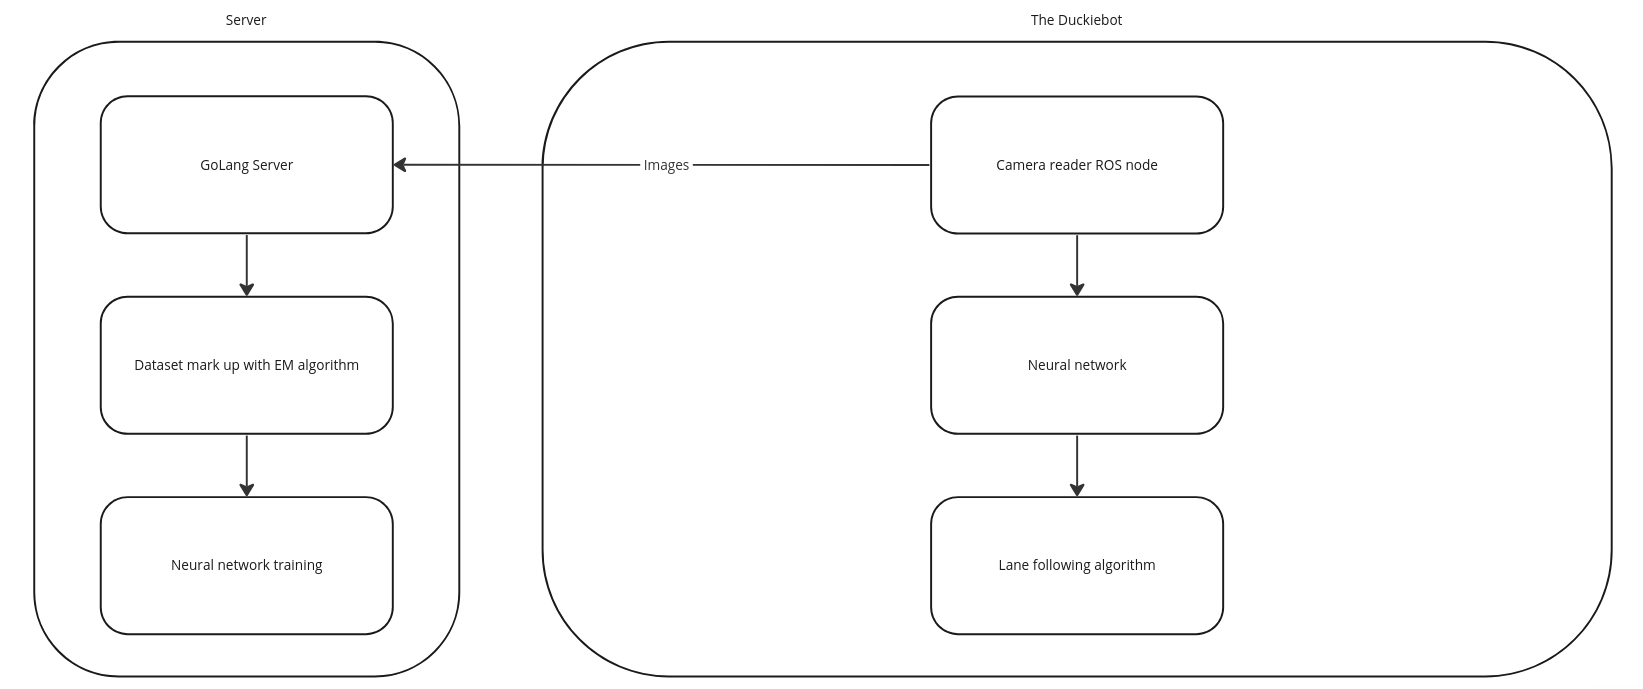
\includegraphics[scale=0.25]{src/Design/assets/ProjectArchitecture.png}
    \caption{Project architecture}\label{project_architecture}
\end{figure}
\subsubsection{Introduction}
As was written in the previous chapter the project was divided into three mini-projects:
\begin{enumerate}
    \item Creating the dataset.
    \item Creating road markup segmentation algorithm.
    \item Deployment of the algorithm on the Duckiebot.
\end{enumerate}
Each mini-project has its own architecture and process flow, however, they were developed in similar environments.
The overall environment is shown in Figure~\ref{project_architecture}. Pictures were collected from the Duckiebot's camera, then they were sent to the GoLang server. 
After that, they were processed in Google Colab and then passed to the neural network training pipeline. During the deployment part images from the same camera on the Duckiebot
were passed to the neural network which had been already deployed on the Duckiebot. And outputs of the neural network were passed to the lane-following algorithm.
\subsubsection{Creating the dataset}
Collecting the dataset involved three steps:
\begin{enumerate}
    \item Developing the infrastructure. The infrastructure includes the ROS node to send data from Duckiebot and the GoLang server to receive and save data. 
    The image was received from the camera and after that, it was sent to the server. Because sending takes some time and this process couldn't be run asynchronously,
    not all images were sent, but every 20.
    \item Collecting the dataset. The collecting of the Dataset was performed manually. The Duckiebot was driven around the road for a few hours. 
    During this process, the lights were changed to collect different data.
    \item Marking up the dataset. The marking up of the Dataset was performed in the Jupiter notebook. Images were marked up in batches of size no more than 500 samples.
    Moreover, pictures of the different light conditions were marked up in different iterations of the pipeline, to prevent noise. After the marking up the dataset was 
    evaluated by humans to remove samples with bad segmentation and after that uploaded to GitHub.
\end{enumerate}
\subsubsection{Creating road markup segmentation algorithm}
\begin{figure}[ht]
    \begin{center}
        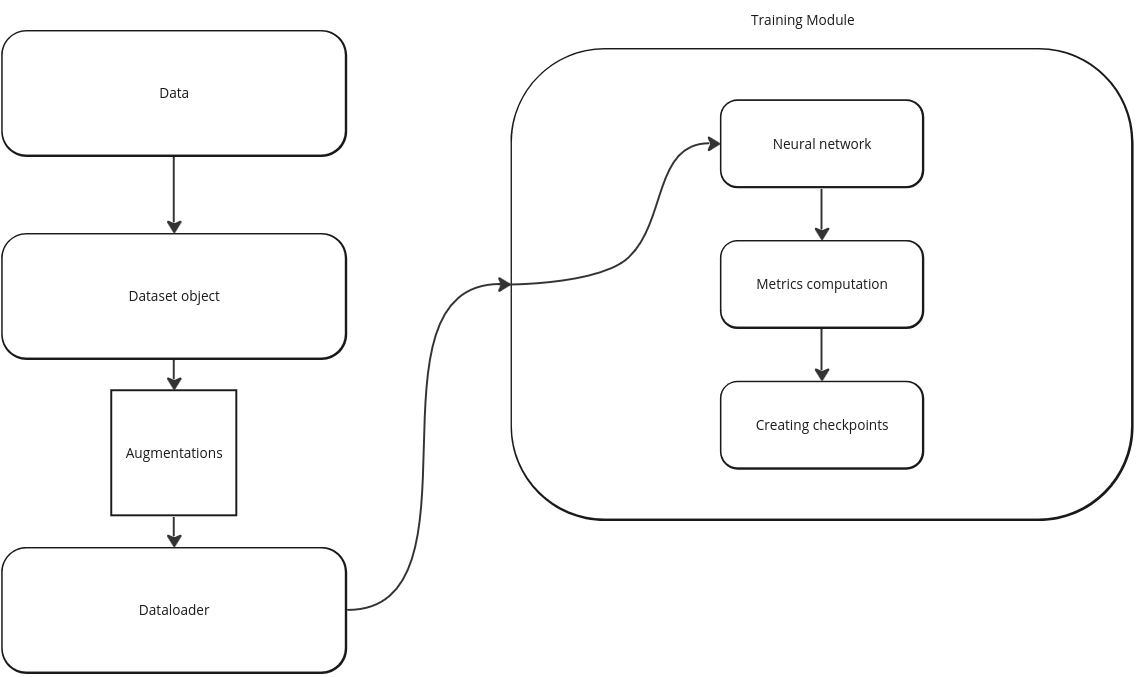
\includegraphics[scale=0.25]{src/Design/assets/TrainingPipeline.png}
    \end{center}
    \caption{Training pipeline}\label{training_pipeline}
\end{figure}
The algorithm was developed in the Jupiter notebook in Google Colab. The pipeline is shown in figure~\ref{training_pipeline}.

The dataset was downloaded from GitHub (it more quicker than uploading it to Colab from a laptop). After that, the data of the dataset was loaded into the dataset class.
The idea of this class is to keep information about the dataset, but not the data itself, because the dataset is pretty huge and keeping all data loaded in the RAM is pretty expensive.
So the Dataset class provides lazy access to the dataset data. If some sample is required it will be loaded, otherwise, only the path to the image will be saved. Also,
the Dataset class is responsible for the augmentation of the data. When a sample is required if this sample is part of the training part of the dataset, then the object 
of the Dataset class will return it with some augmentation, otherwise (if the sample is part of the validation or test part) it will be returned without augmentations.
The Dataset class is used in the Dataloader class. This class is responsible for creating batches of the data and shuffling the test part of the dataset. In this project, it is 
the only functional of the Dataloader class that was used. Whenever the neural network requires a new batch of data, it asks the Dataloader class for it, which uses the Dataset class to load
a few images and provide them to the neural network.

Batches received from the object of the Dataloader class are used in the training and validation of neural network. The TrainingModule class is responsible for this.
This class is developed to make training of the neural network easy. This class has a huge amount of functionality, however, in the project only a few things were used.
The object of the TrainingModule class is responsible for:
\begin{enumerate}
    \item Training the neural network for a few epochs, so the neural network will use in its training each sample of the training part of the dataset a few times.
    \item Calculating metrics during training and validation. It's extremely important because early stopping is used in the training pipeline.
    \item Creating checkpoints of the model. If the target metric of the model doesn't improve after a few epochs the training is finished and a few best iterations are saved.
\end{enumerate}
The overall process flow can be described like this:
\begin{enumerate}
    \item All images saved in Google Colab. All paths are saved in RAM.\@
    \item When an image is required for training or validation it is loaded into RAM.\@ If the image is part of the training part of the dataset augmentations are applied to it.
    \item Required images are combined into a batch.
    \item The batch is fed to the neural network.
    \item The metrics of the batch are computed.
    \item Weights of the neural network are adjusted based on metrics.
    \item When all images of the training part of the set are used (it's called epoch), the images of the validation part are fed to the neural network.
    \item The metrics of the validation part are computed.
    \item If the metrics of validation part don't improve after a few epochs training stops.
    \item The neural network is validated on the test part of the dataset. 
\end{enumerate}

\subsubsection{Deployment}
\begin{figure}[ht]
    \begin{center}
        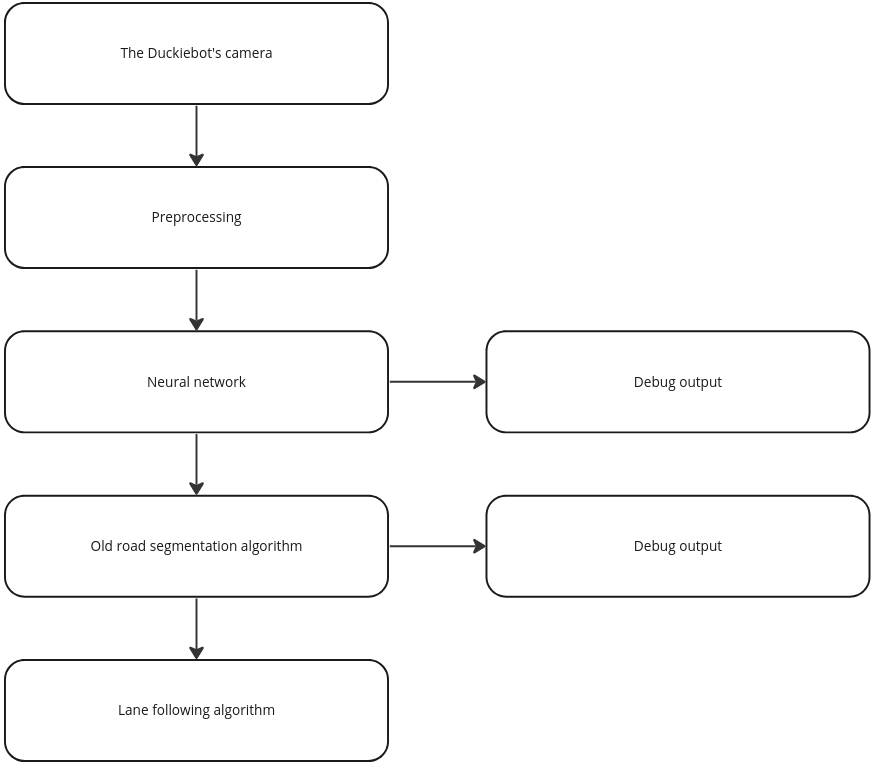
\includegraphics[scale=0.25]{src/Design/assets/Deployment.png}
    \end{center}
    \caption{Deployment}\label{deployment}
\end{figure}
The resulting architecture that is used on the Duckeibot is shown in figure~\ref{deployment}. The image received from the camera of the Duckiebot is preprocessed.
The upper part of the image is removed, because usually it doesn't contain road. After that image is converted to a torch-GPU-tensor. Then this tensor is fed to the neural network.
The output of the neural network is fed into the old lane segmentation algorithm, to convert the output of the neural network to the input of the lane-following algorithm.
The result is fed to the lane-following algorithm, which controls the Duckiebot's movements based on the road markup.

It was decided to use the old lane segmentation algorithm to increase the speed of the development and reduce the risk of creating bugs. However, the old algorithm isn't
fully used. Only the part that is responsible for converting the pixel map to a special input format of the lane-following algorithm is used. The part of creating pixel 
map is removed, because this functionality is taken by the neural network, which was the initial goal of the project.

Also important to mention that the output of the neural network (pixel map) and old lane segmentation (segments of road markup) are sent to a special debug ROS node, which can 
visualize in real-time the images produced by these algorithms. To create these pictures some time is required, so if the debug node isn't used 
(the window with debug information isn't opened) these images won't be sent, which saves some time.
\subsection{EM algorithm}
\subsubsection{Simple case}
Assume there are some amount of points in d-dimensional space, they are samples. The task is to segment them.
\begin{figure}[ht]
    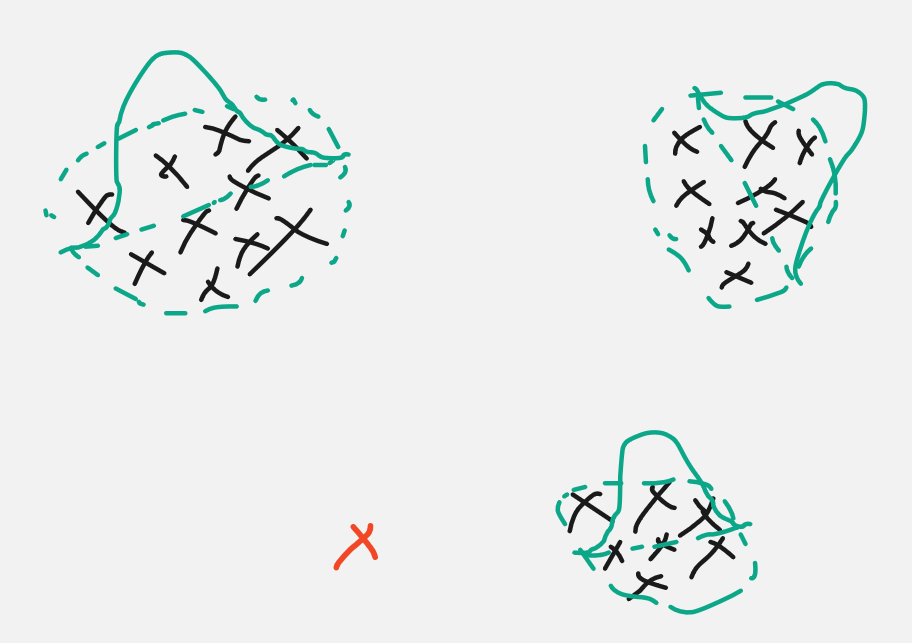
\includegraphics[scale=0.5]{src/Design/assets/em_picture.png}
    \caption{Data visualisation}
\end{figure}
Assume that the picture above is generated by a mixture of three Gaussians.
\[p(\overline{x}) = \pi_1\cdot p_1(\overline{x}) + \pi_2\cdot p_2(\overline{x}) + \pi_3\cdot p_3(\overline{x}) \]
where
\[\sum\limits_{k=1}^{K} \pi_k = 1 \text{ where } K=3\]
In other words, with probability $\pi_i$ Gaussian is chosen and after that, the sample is generated based on this Gaussian 
$\overline{x} \sim p_k(\overline{x})$.
But how to classify a new point (the red one)?
The likelihood function is required:
\[p(D|\overline{\theta}) = \prod\limits_{n=1}^N p(\overline{x}_n | \overline{\theta}) \text{ here D means whole dataset, in other words } D = \{\overline{x}_n \} _{n=1}^N\]
Where
\[p(\overline{x} | \overline{\theta}) = \sum\pi_k\cdotp_k(\overline{x}) = \sum\limits_{k}\pi_k\cdot\mathcal{N}(\overline{x}|\overline{\mu}_k, \Sigma_k)\]
\[\text{Where } \overline{\mu}_i \text{ and } \Sigma_i \text{ are parameters of PDF of normal distribution and } \overline{\theta} = (\pi_1, \dots \pi_K,
\overline{\mu}_1, \Sigma_1, \dots, \overline{\mu}_K, \Sigma_K)\] 
So after that:
\[p(D|\overline{\theta}) = \prod\limits_{n=1}^N p(\overline{x}_n | \overline{\theta}) =
 \prod\limits_{n=1}^N (\pi_1\cdot p_1(\overline{x}_n | \overline{\theta}_1) + \pi_2\cdot p_2(\overline{x}_n | \overline{\theta}_2) + 
 \dots + \pi_K\cdot p_K(\overline{x}_n | \overline{\theta}_K) ) \overset{}{\underset{\overline{\theta}}{\rightarrow}} \text{max}\]
 Where $\overline{\theta}_i = (\overline{\mu}_i, \Sigma_i)$

The problem is that it is a multiplication of a big amount of sums which is difficult to optimize.
The idea is to look at the distribution, likelihood and generation process and think about what other information about this process is required to make 
the likelihood function easy to optimize.

It turns out that adding to the $\overline{x}$ label of its class makes everything much easier. In math terms:
\[ Z = \{\overline{z}_n \} _{n=1}^N \text{, where each } \overline{z}_n \text{ is one-hot encoded: } \overline{z}_n = (0,\dots,1,\dots0)\] 
and only 1 of this vector is on the kth position, which means that $x_n \in C_k$, where $C_k$ means cluster number k.
So if $Z$ is known, then 
\[p(D, Z | \overline{\theta}) = \prod\limits_{n=1}^{N}p(\overline{x}_n, \overline{z}_n | \overline{\theta})
= \prod\limits_{n=1}^{N}p(\overline{z}_n | \overline{\pi})\cdot p(\overline{x}_n| \overline{z}_n, \overline{\theta})
= \prod\limits_{n=1}^{N}\prod\limits_{k=1}^{K}{(\pi_k\cdot\mathcal{N}(\overline{x}_n|\overline{\mu}_k,\Sigma_k))}^{{z_n}_k}\]
Now it's good practice to take the logarithm of likelihood function because it transforms the product into a sum which is a more convenient operation to work with
\[\log(p(D, Z | \overline{\theta})) = \sum\limits_{n=1}^{N}\sum\limits_{k=1}^{K}{z_n}_k \cdot (\log(\pi_k) +  \log(\mathcal{N}(\overline{x}_n|\overline{\mu}_k,\Sigma_k)))
= \sum\limits_{k=1}^K \log(\pi_k) \cdot \sum\limits_{n=1}^N {z_n}_k + 
\sum\limits_{k=1}^K \big( \sum\limits_{n=1}^N {z_n}_k \cdot \log(\mathcal{N}(\overline{x}_n|\overline{\mu}_k,\Sigma_k)) \big)\]
Now important to notice that the first and the second summands depend on different parameters.
The first summand depends on $\pi_k$, while the second depends on parameters of PDF of normal distribution $\overline{\mu}_k, \Sigma_k$. So it's possible to optimize these summands separately.

And now the main idea. There is a complicated likelihood function with latent variables that are not known, but if they were everything would be easy. 
So the idea is to split the process into two steps:
\begin{enumerate}
    \item E-step (fix $\overline{\theta}$, find $\mathbb{E}[Z]$):
    \[\mathbb{E}[z_{n, k}] = p(C_k|\overline{x}_n,\overline{\theta}) 
    = \displaystyle \frac{p(C_k|\overline{\theta})\cdot p(\overline{x}_n|C_k,\overline{\theta})}{\sum\limits_{l=1}^K p(C_l|\overline{\theta})\cdot p(\overline{x}_n|C_l,\overline{\theta})}
    = \displaystyle \frac{\pi_k\cdot \mathcal{N}(\bar x_n | \bar \mu_k, \Sigma_k)}{\sum\limits_{l=1}^K \pi_l \cdot \mathcal{N}(\bar x_n | \bar \mu_l, \Sigma_l)}\]
    \item M-step (fix $\mathbb{E}[Z]$, maximize $\mathbb{E}[\log(p(D,Z|\overline{\theta}))]$). In most cases, instead of $Z$, we can use soft estimates $\mathbb{Z}$:
    \[\mathbb{E}[\log p(D,Z|\bar\theta)] 
    = \mathbb{E}\Big[\sum\limits_n\sum\limits_k {z_n}_k \cdot \big(\log(p(\overline{x}_n|\overline{\mu}_k, \Sigma_k)) + \log(\pi_k)\big)\Big]\] 
    \[ = \sum\limits_n\sum\limits_k\mathbb{E}[{z_n}_k]\cdot(\log(\pi_k) + \log\big(p(\overline{x}_n|\overline{\mu}_k, \Sigma_k))) \newline
    = \sum\limits_k\Big(\sum\limits_n\mathbb{E}[z_{n,k}]\Big) \log \pi_k + \sum\limits_k\sum\limits_n\mathbb{E}[z_{n,k}]\cdot \log p(\bar x_n|\bar\mu_k,\Sigma_k)\]
\end{enumerate}

\subsubsection{General case}
There are:
\begin{enumerate}
    \item X \- the dataset
    \item Z \- latent variables we don't know them
    \item $\theta$ \- parameters we also don't know them
\end{enumerate}
The goal is to maximize $p(X|\theta)$, which is a complicated task, but optimizing $p(X, Z|\theta)$ is easier. So let
\[Q(\theta, \theta^{(n)}) := \mathbb{E}_{p(Z|X,\theta^{(n)})} \big[\log p(X,Z|\theta)\big]
= \int \log p(X,Z|\theta) \cdot p(Z|X,\theta^{(n)}) dz \]
And on each step:
\[\theta^{(n+1)} = \underset{\theta}{argmax}Q(\theta, \theta^{(n)})\]

These steps are executed until $\theta$ stops changing or the likelihood function stops changing (theoretically it should happen simultaneously). 
Also, the likelihood function should increase after each step. So in the end:
\[\log(p(X|\theta)) > \log(p(X|\theta^{(n)}))\]
\[\log(p(X|\theta)) - \log(p(X|\theta^{(n)})) 
= \log \Big( \int p(X,Z|\theta) dz \Big) - \log(p(X|\theta^{(n)})) \]
\[= \log \Big(\int p(Z|X,\theta^{(n)} \cdot \displaystyle \frac{p(X,Z|\theta)}{p(Z|X,\theta^{(n)})}) dz \Big) - \log(p(X|\theta^{(n)}))\]
\[= \log\Big( \mathbb{E}_{p(Z|X,\theta^{(n)})}\big[\displaystyle\frac{p(X,Z|\theta)}{p(Z|X,\theta^{(n)})} \big] \Big) - \log(p(X|\theta^{(n)})) \]
\[ \underset{\text{by the Jensen's inequality}}{\geq} \mathbb{E}_{p(Z|X,\theta^{(n)})}\Big[\log\big(\displaystyle\frac{p(X,Z|\theta)}{p(Z|X,\theta^{(n)})} \big) \Big]  - \log(p(X|\theta^{(n)})) \]
\[ = \mathbb{E}_{p(Z|X,\theta^{(n)})}\Big[\log\big(\displaystyle\frac{p(X,Z|\theta)}{p(Z|X,\theta^{(n)}) \cdot p(X|\theta^{(n)})} \big) \Big]\]
Now important to notice, that $p(Z|X,\theta^{(n)}) \cdot p(X|\theta^{(n)}) = p(X,Z|\theta^{(n)})$

\noindent And therefore:
\[ \log(p(X|\theta)) \geq \log(p(X|\theta^{(n)})) + \mathbb{E}_{p(Z|X,\theta^{(n)})}\Big[\log\big(\displaystyle\frac{p(X,Z|\theta)}{p(Z|X,\theta^{(n)}) \cdot p(X|\theta^{(n)})} \big) \Big] =: \mathcal{L}(\theta, \theta^{(n)})\]

\begin{figure}[h]
    \begin{center}
        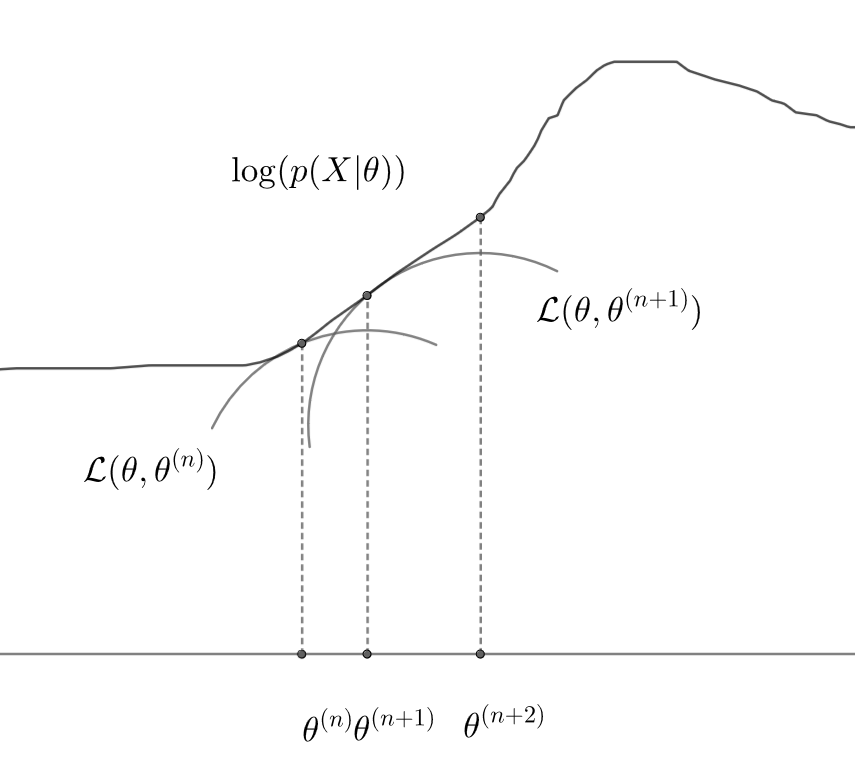
\includegraphics[scale=0.45]{src/Design/assets/em_visualisation.png}
    \end{center}
    \caption{Algorithm visualisation}
\end{figure}

As shown in the picture in each point ($\theta^{(n)}$, $\theta^{(n+1)}$, $\theta^{(n+2)}$, etc) the lower score of $\log(p(X|\theta))$ is known. This score is $\mathcal{L}(\theta, \theta^{(n)})$

Also, it's important to mention that $\log(p(X|\theta^{(n)})) = \mathcal{L}(\theta^{(n)}, \theta^{(n)})$

So the idea is to optimize $\mathcal{L}(\theta, \theta^{(n)})$. The function converges to a local maximum which is also good.

But in the beginning, it was said that $Q(\theta, \theta^{(n)})$ needs to be optimized, it turns out that in terms of optimization $Q$ and $\mathcal{L}$ 
are the same functions.

\[ \mathcal{L}(\theta, \theta^{(n)}) = \underset{const(\theta)}{\log(p(X|\theta^{(n)}))} + \underset{\text{it is } Q(\theta, \theta^{(n)})}{\mathbb{E}_{p(Z|X,\theta^{(n)})}\Big[\log\big(p(X,Z|\theta) \big) \Big]}
- \underset{const(\theta)}{\mathbb{E}_{p(Z|X,\theta^{(n)})}\Big[\log\big(p(X,Z|\theta^{(n)})\big)\Big]}
    \]

\subsection{Deep learning model}
\subsubsection{Architecture}
\begin{figure}[h]
    \begin{center}
    \subfloat[Full model architecture]{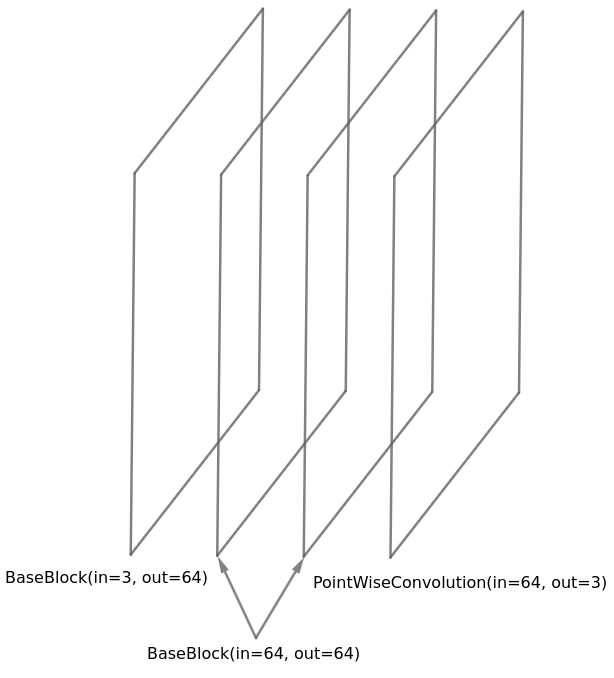
\includegraphics[scale=0.35]{src/Design/assets/nn_architecture.png}}
    \subfloat[Basic block architecture]{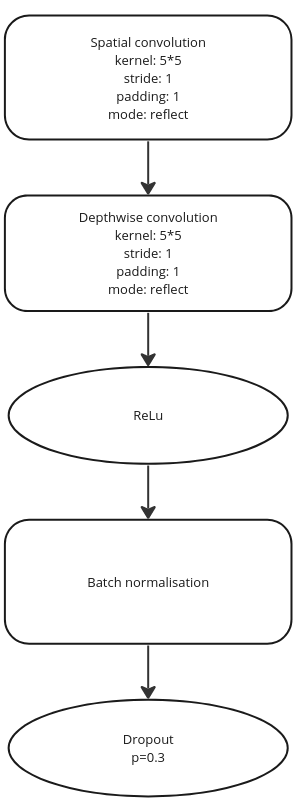
\includegraphics[scale=0.45]{src/Design/assets/basic_block_architecture.png}}
    \end{center}
    \caption{The DL model architecture}\label{nn_architecture}
\end{figure}
The architecture of the model is shown in Figure~\ref{nn_architecture}. The idea of MobileNet~\cite{mobileNet} for splitting the convolutional layer into two parts 
was used to increase the speed of the neural network.
As the loss function, the cross-entropy function was used.
\[ \mathcal{L}(x,y) = \{l_1,\dots,l_n\}; l_n=-w_{y_n}\log\frac{e^{x_{n,y_n}}}{\sum\limits_{c=1}^C e^{x_{n,c}}}\]
\[\text{ where } x\in \mathbb{R}^{n\times C} \text{ are outputs of the model}
\text{ and } y \in \mathbb{N}^n \text{ are ground truth class labels for each sample} \]

For the road markup segmentation task, this architecture was enough. Scores of the model are shown in the Implementation chapter. 
Each layer is described in more detail below.
\subsubsection{General neural networks ideas}
\begin{figure}[h]
    \begin{center}
    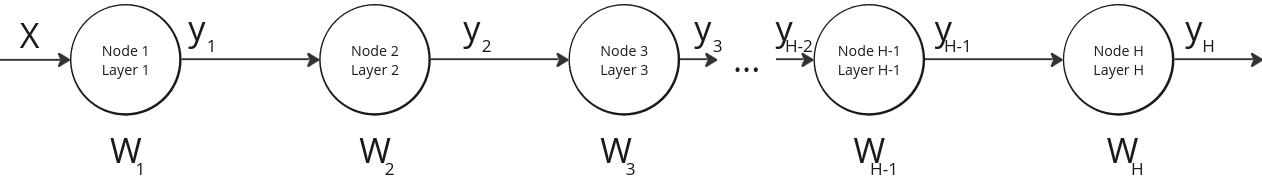
\includegraphics[scale=0.35]{src/Design/assets/computational_graph.png}
    \end{center}
    \caption{Computational graph}\label{com_graph}
\end{figure}
To talk about convolutional neural networks it's important to discuss the idea of neural networks in general.

Each neural network can be represented as a computational graph. The first node of the graph is the input and the last is the output of the network.
The output of the neural network (in formulas $\hat{y}$ is used) passes to the loss function. Almost always the task of training is to minimize the loss function.
To do this backpropagation is used.
Let $X \in \mathbb{R}^{n\times d}$ is input of the neural network, $\hat{y}\in \mathbb{R}^{n\times k}$ is output, $\{\hat{y}_i \in \mathbb{R}^{n \times k_i}\} _{i=1}^{H}$ 
is the output of the ith layer (or node in terms of the graph) of the neural network and $y \in \mathbb{R}^{n\times m}$ is a vector of ground truth answers 
(real numbers, class labels, etc). Also each layer has weights $\{ w_i \in \mathbb{R}^{k_i} \} _{i=1}^{H}$ (bias is included in weights for convenience) 
Here $n$ is used as the size of a dataset used for training and $H$ is the number of layers of a neural network (or nodes in terms of a graph)

In the described terms backpropagation can be described like this:
\begin{itemize}
    \item $\displaystyle\frac{\partial L}{\partial \hat{y}} =: \frac{\partial L}{\partial y_H}$ is the partial derivative of the loss function by the output of the neural network
    \item $\displaystyle \forall i \in \{1\dots H-1\}\text{ } \frac{\partial L}{\partial y_i} = \frac{\partial L}{\partial y_{i + 1}} \cdot \frac{\partial y_{i + 1}}{\partial y_i}$
\end{itemize}
The training is an iterative process, so $w_i^{(j)}$ mean weights of layer $i$ on the jth iteration of the process. The process can be described like this:
\begin{itemize}
    \item $\displaystyle \forall i \in \{2\dots H\} \text{ }w_i^{(j+1)} = w_i^{(j)} - \eta \cdot \frac{\partial L}{\partial w_i} \Big|_{w_i^{(j)}, y_{i-1}}$
    \item $\displaystyle w_1^{(j+1)} = w_1^{(j)} - \eta \cdot \frac{\partial L}{\partial w_1} \Big|_{w_1^{(j)}, X}$
\end{itemize}

All gradients and things specific to each layer used in the provided architecture are listed below

\subsubsection{Convolutional layer}
The convolutional layer is called this way because this layer performs a math transformation called convolution:
\[(f * g)(x) := \int\limits_{\mathbb{R}^n}f(x-y)g(y)dy= \int\limits_{\mathbb{R}^n}f(y)g(x-y)dy\]
However, in convolutional neural networks (CNN) this operation is usually performed iteratively because it's more efficient.
To implement the convolutional layer iteratively the sliding window is used.

Let $X \in \mathbb{R}^{N\times D \times H \times W}$ be the batch of input images (or feature maps) if it is an image $D$ usually equals $3$ and means the number of colors channels, 
$W$ and $H$ are the widths and the heights of the image or feature map and $N$ is the batch size (amount of samples of training set simultaneously fed to a neural network in 
a single forward pass).
$K = \in \mathbb{R}^{L \times D \times H_k \times W_k}$, where $W_k = 2\cdot a+1$ and $H_k = 2\cdot b+1$ is the kernel (sliding window).

The convolution of $X$ and $K$ ($X*K$) is another tensor $Y\in \mathbb{R}^{N\times L\times W' \times H'}$, where~\cite{conv2dTorch} 
\[
    W' = \displaystyle \Big\lfloor\frac{W  + 2 \cdot p_1 - d_1 \cdot (W_k - 1) - 1}{s_1} + 1\Big\rfloor    
\]
\[
    H' = \displaystyle \Big\lfloor\frac{H  + 2 \cdot p_0 - d_0 \cdot (H_k - 1) - 1}{s_0} + 1\Big\rfloor       
\]

\begin{figure}[h]
    \begin{center}
    \subfloat[Padding = 1]{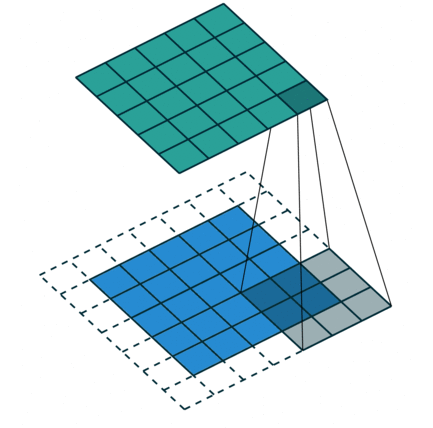
\includegraphics[scale=0.35]{src/Design/assets/padding.png}}
    \subfloat[Dilation = 2]{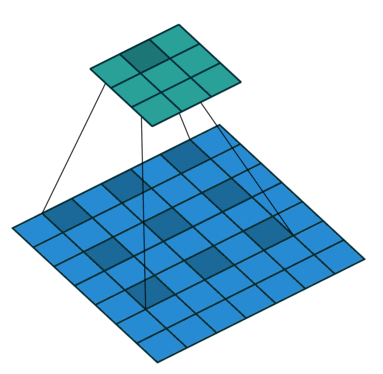
\includegraphics[scale=0.45]{src/Design/assets/dilation.png}}
    \\
    \subfloat[Stride = 2 (a)]{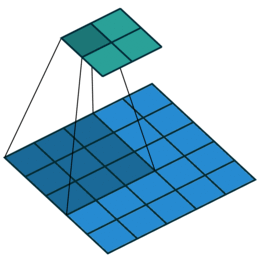
\includegraphics[scale=0.45]{src/Design/assets/stride1.png}}
    \subfloat[Stride = 2 (b)]{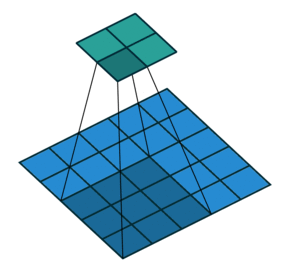
\includegraphics[scale=0.45]{src/Design/assets/stride2.png}}
    \end{center}
    \caption{Visualisation of convolution layer parameters}\label{conv2dparams}
\end{figure}

\begin{itemize}
    \item $p_i$ padding of spatial dimensions of the input tensor
    \item $d_i$ is dilation. Spacing between kernel elements
    \item $s_i$ is stride. A stride of the convolution
\end{itemize}

The visualisation of each parameter is shown on Figure~\ref{conv2dparams}~\cite{conv2dParamsArticle}

The elements of the result tensor are computed in the following way:
\[
    Y_{n, k, h, w} = \sum\limits_{d=0}^{D}\sum\limits_{j=-\lfloor W_k / 2\rfloor}^{\lfloor W_k / 2\rfloor}\sum\limits_{i=-\lfloor H_k / 2\rfloor}^{\lfloor H_k / 2\rfloor}
    X_{n, d, h \cdot s_0 + i \cdot d_0, w \cdot s_1 + j \cdot d_1} \cdot K_{k, d, i + \lfloor H_k / 2\rfloor, j + \lfloor W_k / 2\rfloor}
\]

The gradients of this layer can be computed like this (only the most common case, where $\displaystyle p_0 = \Big\lfloor \frac{H_k}{2} \Big\rfloor$, $\displaystyle p_1=\Big \lfloor \frac{W_k}{2} \Big\rfloor$ 
and $s_0 = s_1 = d_0 = d_1 = 1$ is considered because only this case was used in the project's architecture, important to notice that in this case $W'=W$ and $H'=H$):
\begin{itemize}
    \item To compute $\frac{\partial L}{\partial X}$ it's need to define $\widehat{K} \in \mathbb{R}^{D \times L \times W_k \times H_k}: \text{ } \widehat{K}_{d,l,w,h} = K_{l,d,h,w}$
    \[
        \displaystyle \frac{\partial L}{\partial X} = \frac{\partial L}{\partial Y} * \widehat{K}
    \]

    \item Some kind of convolution is also used to calculate $\frac{\partial L}{\partial K}$, but summation takes place by the size of the batch, not by channels 
    \[
        \frac{\partial L}{\partial K}_{l, d, h, w} = \sum\limits_{n=0}^N\sum\limits_{i=0}^H\sum\limits_{j=0}^W X_{n,d,i+h-\lfloor \frac{H_k}{2} \rfloor, j+w-\lfloor \frac{W_k}{2} \rfloor}
        \cdot \frac{\partial L}{\partial Y}_{n, l, i, j}
    \]
\end{itemize}

\textbf{Important notice} \\
$X_{i,-1,-1}$ is valid notation. It means that padded values are used. The mode of padding can be different in this project reflect mode is used.

\subsubsection{Batch normalisation layer}
This type of layer was first introduced in 2015 in this paper~\cite{batch_norm}.
This layer is used to keep all data in a neural network in one type of distribution. This technique prevents gradient explosions and 
helps a neural network to converge faster.
The idea of the batch normalization layer is pretty simple. During training update count mean and variance for the batch and apply it to training data and during inference just 
apply running estimates of those values to the data.

The forward pass of the layer during training can be described in the following way:
\begin{enumerate}
    \item Count batch statistics:
    \begin{itemize}
        \item $\mu = \displaystyle \frac{1}{m} \sum\limits_{i=1}^m x_i$
        \item $\sigma^2 = \displaystyle \frac{1}{m} \sum\limits_{i=1}^m (x_i - \mu) ^ 2$
    \end{itemize}
    \item Normalize the batch: $\hat{x_i} = \displaystyle \frac{x_i - \mu}{\sqrt{\sigma^2 + \varepsilon}}$
    \item Scale the batch: $y_i = \gamma \cdot \hat{x_i} + \beta$, where $\gamma$ and $\beta$ are trainable parameters
\end{enumerate}

During inference instead of $\mu$ and $\sigma^2$ $E[x]$ and $VAR[x]$ are used which were calculated during training.

Gradients of this layer are pretty simple:
\begin{enumerate}
    \item $\displaystyle \frac{\partial L}{\partial \hat{x}_i} = \frac{\partial L}{\partial y_i} \cdot \gamma$
    \item $\displaystyle \frac{\partial L}{\partial \sigma^2} = \sum\limits_{i=1}^m \frac{\partial L}{\partial \hat{x}_i} \cdot (x_i - \mu) \cdot \frac{-1}{2} \cdot
    {(\sigma^2+\varepsilon)}^{\frac{-3}{2}}$
    \item $\displaystyle \frac{\partial L}{\partial \mu} = \Big(\sum\limits_{i=1}^m \frac{\partial L}{\partial \hat{x}_i} \cdot \frac{-1}{\sqrt{\sigma^2 + \varepsilon}}\Big)
    + \frac{\partial L}{\partial \sigma^2 } \cdot \frac{\sum\limits_{i=1}^m -2(x_i-\mu)}{m}$
    \item $\displaystyle \frac{\partial L}{\partial x_i} = \frac{\partial L}{\partial \hat{x}_i} \cdot \frac{1}{\sqrt{\sigma^2 + \varepsilon}} +
    \frac{\partial L}{\partial \sigma^2} \cdot \frac{2(x_i-\mu)}{m} + \frac{\partial L}{\partial \mu} \cdot \frac{1}{m}$ 
    \item $\displaystyle \frac{\partial L}{\partial \gamma} = \sum\limits_{i=1}^m\frac{\partial L}{\partial y_i} \cdot \hat{x}_i$
    \item $\displaystyle \frac{\partial L}{\partial \beta} = \sum\limits_{i=1}^m\frac{\partial L}{\partial y_i}$
\end{enumerate}

\subsubsection{ReLu activation}
ReLu is used in the project's architecture as an activation function. This function proved itself to be a good activation and some kind of baseline in modern deep learning~\cite{relu}
\[
ReLu(x) = y =
\begin{cases}
    0 & \text{if } x \leq 0 \\
    x & \text{if } x > 0
\end{cases}    
\]
The gradient of ReLu is obvious:
\[
\frac{\partial L}{\partial x} = 
\begin{cases}
    0 & \text{ if } x \leq 0 \\
    \frac{\partial L}{\partial y} & \text{ if } x > 0
\end{cases}    
\]

\subsubsection{Dropout layer}
\begin{figure}[h]
    \begin{center}
    \subfloat[Standard neural network]{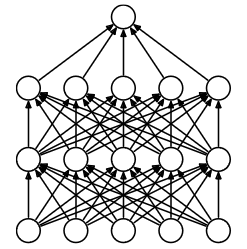
\includegraphics[scale=0.35]{src/Design/assets/before_dropout.png}}
    \subfloat[After dropout]{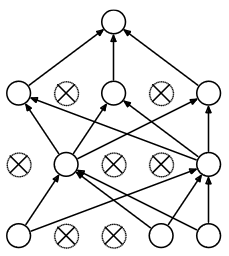
\includegraphics[scale=0.45]{src/Design/assets/after_dropout.png}}
    \end{center}
    \caption{Dropout layer}\label{dropout_layer}
\end{figure}
% The dropout layer is used in NN as a method of regularization to prevent overfiting~\cite{dropout}.
% This layer breaks connections between layers for some parts of the data. The gradients of these elements are equal to zero.
The main idea of Dropout is to randomly and temporarily exclude neurons from the network during training. At the same time, 
each neuron has the probability of being "turned off" at each iteration of network training. This forcibly makes the network 
less capable of memorizing specific patterns, which helps the network generalize its knowledge to new data.

Using Dropout usually improves the generalizing ability of the model and prevents overfitting, especially in cases where the 
training sample is small or when the model has a large number of parameters.

If usually neural network works like this:
\begin{enumerate}
    \item $\overline{z}^{(l)} = \overline{w}^{(l)}\cdot \overline{y}^{(l-1)}$
    \item $\overline{y}^{(l)} = f(\overline{z}^{(l)})$
\end{enumerate}
With the dropout layer, its behavior can be described in the following way:
\begin{enumerate}
    \item $r^{(l)} \sim Bernoulli(p)$
    \item $\tilde{y}^{(l)} = r^{(l)} \odot y^{(l)}$, where $\odot$ means element-wise multiplication
    \item $\overline{z}^{(l)} = \overline{w}^{(l)}\cdot {\tilde{y}}^{(l-1)}$
    \item $\tilde{y}^{(l)} = f(\overline{z}^{(l)})$
\end{enumerate}

\subsubsection{Optimizers}
As was written above in neural networks updating weights can be implemented in the following way:
\[W^{(n)} = W^{(n-1)} - \eta \nabla_W \mathcal{L}(W^{(n-1)}, X, y)\]
Where $W$ is the tensor with model weights, $X$ is the input tensor and $y$ is the ground truth tensor.

However, this approach has some disadvantages~\cite{sgd}:
\begin{enumerate}
    \item Convergence problem, using classical stochastic gradient descent (SGD) usually doesn't guarantee good convergence.
    \item Learning rate should be chosen wisely and updated during training.
    \item The same learning rate is applied to all weights, which can be a problem since not all weights are in the same distribution and scale.
    \item SGD can lead to a local minimum of a loss function, which sometimes can cause problems during inference.
\end{enumerate}
To solve these problems a lot of different approaches for updating weights were invented. In this project, two of them were tried and one of them was finally used.

\textbf{SGD Momentum}

SGD encounters challenges when navigating through ravines, where the terrain of gradient sharply curves in one dimension more than another, 
often found near local optima. In such cases, SGD tends to zigzag along the slopes of the ravine, making slow progress toward the local optimum. 

Momentum, however, addresses this issue by accelerating SGD in the direction of relevance while dampening oscillations. 
This is achieved by incorporating a fraction of the update tensor from the previous time step into 
the current update tensor. 
\[v^{(n)}=\gamma \cdot v^{(n-1)} + \eta \nabla_W \mathcal{L}(W^{(n-1)}, X, y)\]
\[W^{(n)} = W^{(n-1)} - v ^{(n)}\]
$\gamma \cdot v^{(n-1)}$ is called momentum. It is usually set to $0.9$~\cite{sgd}. 

In other words, parameter updates accumulate momentum, accelerating convergence where gradients coincide and reducing measurement updates with 
varying gradients. Consequently, the pulse promotes faster convergence and mitigates fluctuations.

\begin{figure}[h]
    \begin{center}
    \subfloat[SGD without monmentum]{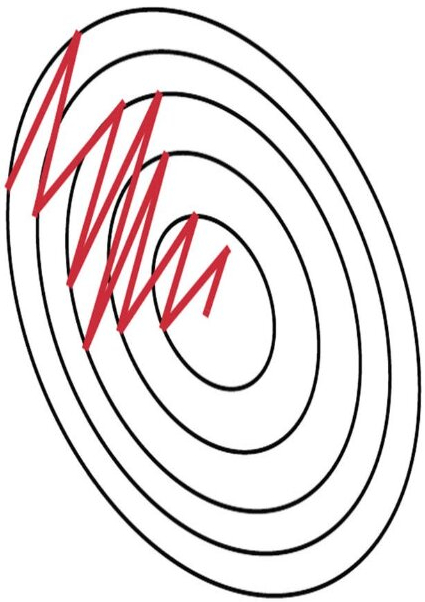
\includegraphics[scale=0.35]{src/Design/assets/sgd.jpg}}
    \subfloat[SGD with momentum]{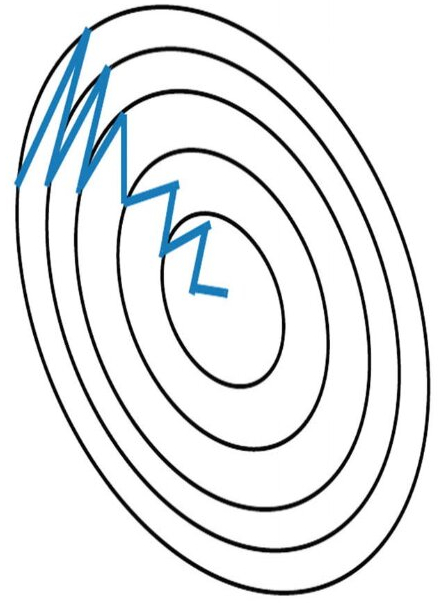
\includegraphics[scale=0.35]{src/Design/assets/sgd_momentum.jpg}}
    \end{center}
    \caption{SGD}\label{SGD}
\end{figure}

\textbf{Adam}

If SGD momentum solves the convergence problem, then Adaptive Moment Estimation (Adam)~\cite{adam} solves other problems, like learning rate scheduling, 
different learning rates for different weights and of course convergence problems. 
The algorithm of Adam can be described below:
\[g^{(n)} = \nabla_{W} \mathcal{L}(W^{(n-1)}, X, y) + \lambda \cdot W^{(n-1)}\]
\[m^{(n)} = \beta_1 \cdot m^{(n-1)} + (1-\beta_1)g^{(n)}, \text{ where } m^{(0)} = 0\]
\[v^{(n)} = \beta_2 \cdot v^{(n-1)} + (1-\beta_2){(g^{(n)})}^2 , \text{ where } v^{(n)} = 0\]
\[\widehat{m}^{(n)} = \frac{m^{(n)}}{1 - \beta_1^n}\]
\[\widehat{v}^{(n)} = \frac{v^{(n)}}{1-\beta_2^n}\]
\[W^{(n)} = W^{(n-1)} - \eta \cdot \frac{\widehat{m}^{(n)}}{\sqrt{\widehat{v}^{(n)}} + \varepsilon} \]
Here's $\eta$ is the common learning rate, $\beta_1, \beta_2$ parameters for computing running averages of gradient and its square, 
$\lambda$ is weight decay coefficient, it adds L2 regularisation for the optimizer. Authors of the algorithm suggest to use $\beta_1 = 0.9$, 
$\beta_2 = 0.999$, $\varepsilon = 10^{-8}$

The benefits of Adam are that:
\begin{enumerate}
    \item It computes adaptive learning rates for each parameter
    \item It stores bias-corrected first and second moment estimates of the exponentially decaying average of past gradients
    \item It applies L2 regularisation
\end{enumerate}

Even though Adam uses techniques of SGDM it's not obvious which optimizer is better~\cite{adam_vs_sgd}. It turns out that sometimes SGDM performs better.
That's why both optimizers were tried in the project. The choice and its reason are described in the implementation chapter.

\subsection{General project design}
As it was written in the Project planning chapter the project was divided into three big parts. The code base is shown in Figure~\ref{code_base}
\begin{figure}[h]
    \begin{center}
    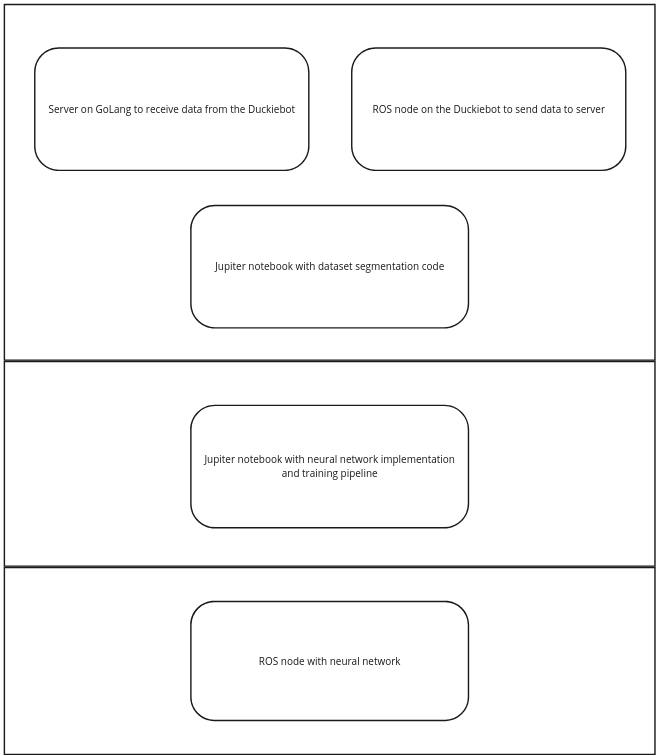
\includegraphics[scale=0.35]{src/Design/assets/code_base.png}
    \end{center}
    \caption{Code base}\label{code_base}
\end{figure}
\subsubsection{The Server}
For the server, it was decided to use a simple socket architecture. 
The server was able to handle multiple requests simultaneously, even though the Duckiebot can't asynchronously send data 
(a new photo was sent to the server only after the previous one was fully sent), writing data to disk was a bit slower than receiving pictures via WiFi. 
So a new request could come before the previous was completed. 
\subsubsection{Jupiter notebooks}
The use of Jupiter notebooks is usually in research projects. 
This technology provides the ability to execute various parts of the code without having to execute the entire pipeline. 
Since writing ML models is divided into analyzing the dataset, writing the model itself, training and testing it, 
the ability to run different parts of the code, saving variables and states after other runs is very useful.
This feature also allows you to abandon writing unit and integration tests at least at the research stage, since in case of an error, 
you can immediately see which part of the code is not working, as well as errors similar to differences in the input format are easily identified and corrected.

In addition to all the described below benefits, Jupiter notebooks are easily convertible to regular Python files, which makes migration from the research stage
to the deployment extremely easy.

\subsubsection{Deployment on the Duckeibot}
The Duckiebot is run under ROS.\@ So to deploy something on it the ROS node should be created. It was decided not to create a new ROS node, but to use the existing one,
which was used for an old lane segmentation algorithm. Moreover, the output of the created algorithm is fed into the part of the old lane segmentation algorithm.
This was done to use already existing and working code to communicate with the lane-following algorithm. However, from old algorithm part with segmentation was 
removed and only the part with converting the color mask to required for lane-following algorithm input was saved.